\chapter{Matplotlib}

\section{Introduction to Matplotlib}
Matplotlib is the foundational plotting library in Python. It is used extensively on its own, and serves as the underlying drawing engine for pandas and Seaborn. The standard import convention is \texttt{import matplotlib.pyplot as plt}.

\subsection{Two Interfaces: Stateful vs. Stateless}
Matplotlib can be used in two distinct ways[cite: 156]:

\begin{figure}[h]
    \centering
    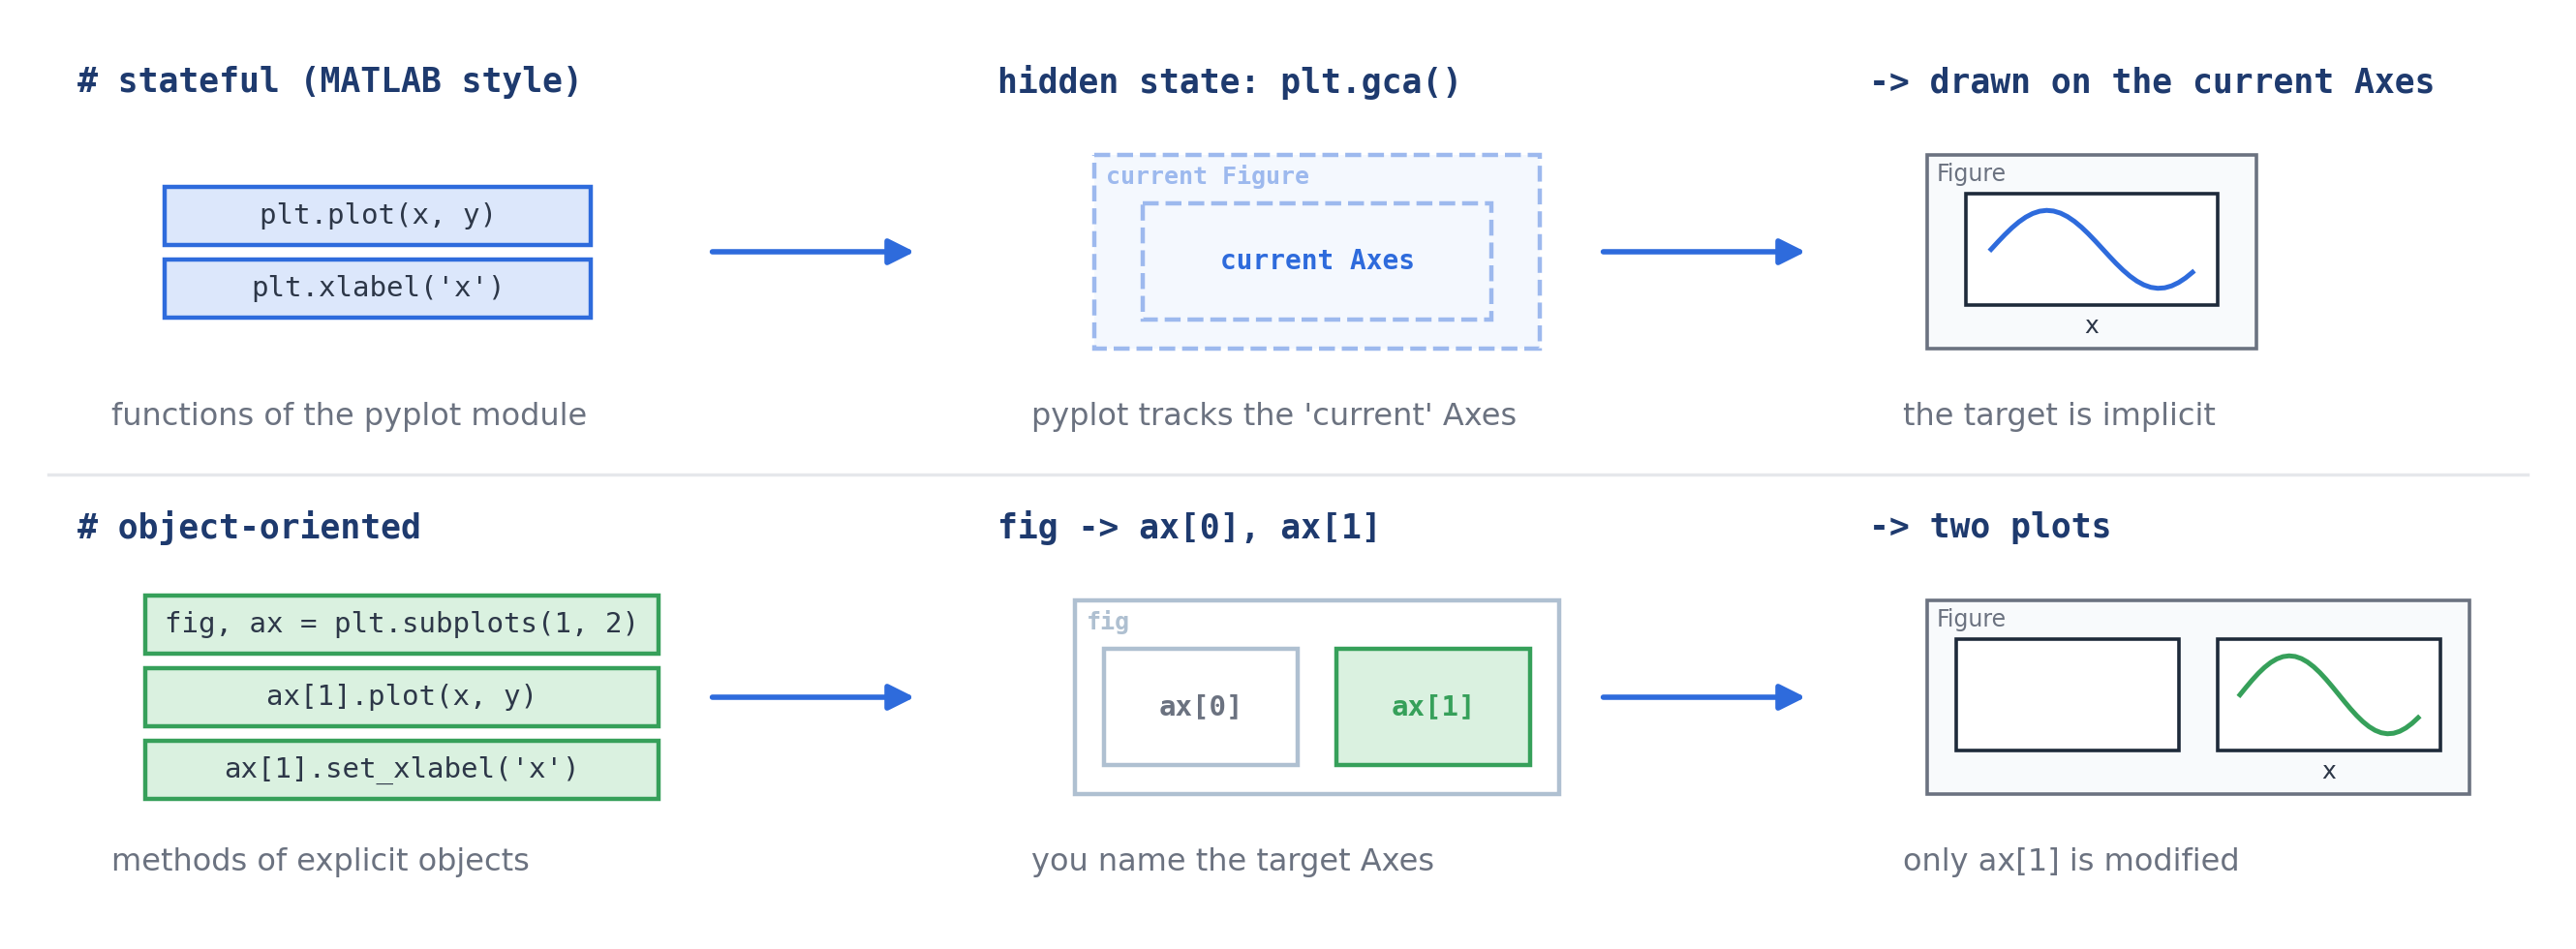
\includegraphics[width=1\textwidth]{contents/images/matplotlib/sub_interfaces.png}
    \caption{The two Matplotlib interfaces: \texttt{pyplot} functions act on the current Axes, tracked implicitly by Matplotlib, while the object-oriented style calls methods on explicit \texttt{Figure} and \texttt{Axes} objects, so the target of each call is always clear.}
\end{figure}

\begin{itemize}
    \item \textbf{Stateful (MATLAB style):} You call functions directly from the \texttt{pyplot} module (e.g., \texttt{plt.plot()}, \texttt{plt.xlabel()}). These functions automatically apply changes to the \textit{current} active Figure and Axes, which Matplotlib tracks in the background.
    \item \textbf{Stateless (Object-Oriented):} You explicitly call methods on specific \texttt{Figure} and \texttt{Axes} objects (e.g., \texttt{ax.plot()}, \texttt{ax.set\_xlabel()}). This approach is strongly recommended because it makes it perfectly clear which plot you are modifying, especially when working with multiple plots at once.
\end{itemize}

\lstinputlisting[caption={Stateful vs. Stateless (Object-Oriented) approaches in Matplotlib.}]{contents/listings/matplotlib/interfaces.py}



\section{Stateless: Figures and Axes}
A \textbf{Figure} is the overall window or image, whereas the \textbf{Axes} are the individual plots contained inside the Figure, each with its own x-axis and y-axis. A single Figure can hold multiple Axes.

\subsection{Creating a Figure and Line Plot}
\begin{itemize}
    \item \texttt{plt.subplots(figsize=(width, height))} creates and returns a new Figure and its associated Axes. The dimensions are specified in inches.
    \item \texttt{ax.plot(x, y)} takes two lists or NumPy arrays containing coordinates and joins the points with line segments. Calling it multiple times on the same Axes automatically adds new lines in different colors.
    \item You can configure the plot's appearance using \texttt{ax.set\_...} methods (e.g., \texttt{ax.set\_xlabel}, \texttt{ax.set\_xlim}, \texttt{ax.set\_xticks}) and add a grid with \texttt{ax.grid()}.
\end{itemize}

\begin{figure}[h]
    \centering
    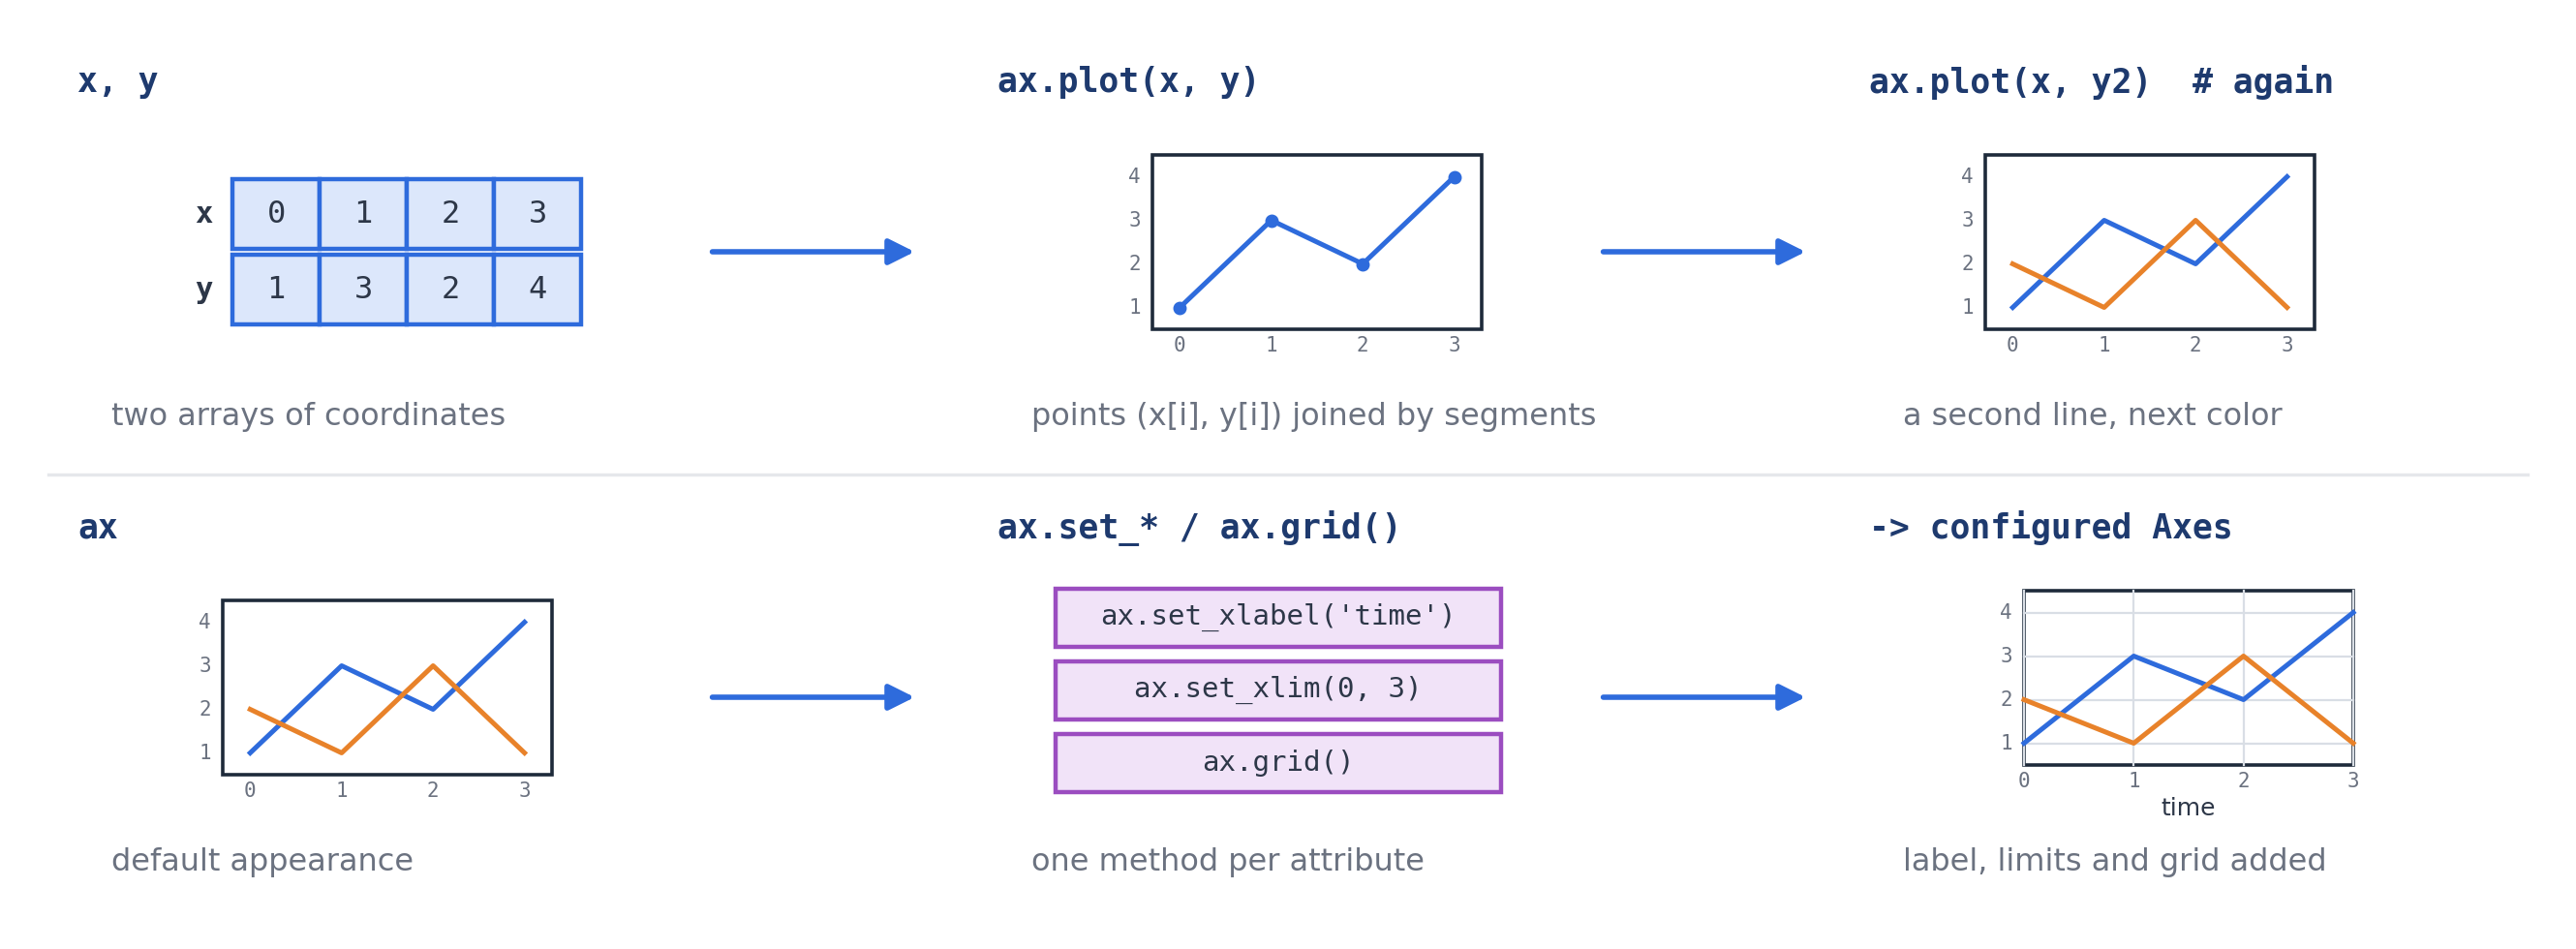
\includegraphics[width=1\textwidth]{contents/images/matplotlib/sub_line_plot.png}
    \caption{Line plots: \texttt{ax.plot(x, y)} joins the points \texttt{(x[i], y[i])} with segments, and each new call adds a line in the next color. The \texttt{ax.set\_...} methods and \texttt{ax.grid()} change one attribute of the Axes at a time.}
\end{figure}

\lstinputlisting[caption={Creating a plot and setting axis attributes using the stateless interface.}]{contents/listings/matplotlib/attributes.py}

\subsection{Creating Many Subplots}
You can create a grid of plots by passing the number of rows and columns as the first two arguments to \texttt{plt.subplots()}.
\begin{itemize}
    \item \textbf{1D Grid:} If you create one row of $n$ Axes, the returned \texttt{ax} object is a 1-D NumPy array of shape \texttt{(n,)}. You access the second plot using \texttt{ax[1]}.
    \item \textbf{2D Grid:} If you create a grid of $m$ rows and $n$ columns, \texttt{ax} is a 2-D array of shape \texttt{(m, n)}. You access the bottom-right plot using coordinate indexing, like \texttt{ax[1, 1]}.
    \item \textbf{Tight Layout:} Always call \texttt{fig.tight\_layout()} at the end of your plotting code to automatically adjust spacing and prevent the labels of neighboring subplots from overlapping.
\end{itemize}

\begin{figure}[h]
    \centering
    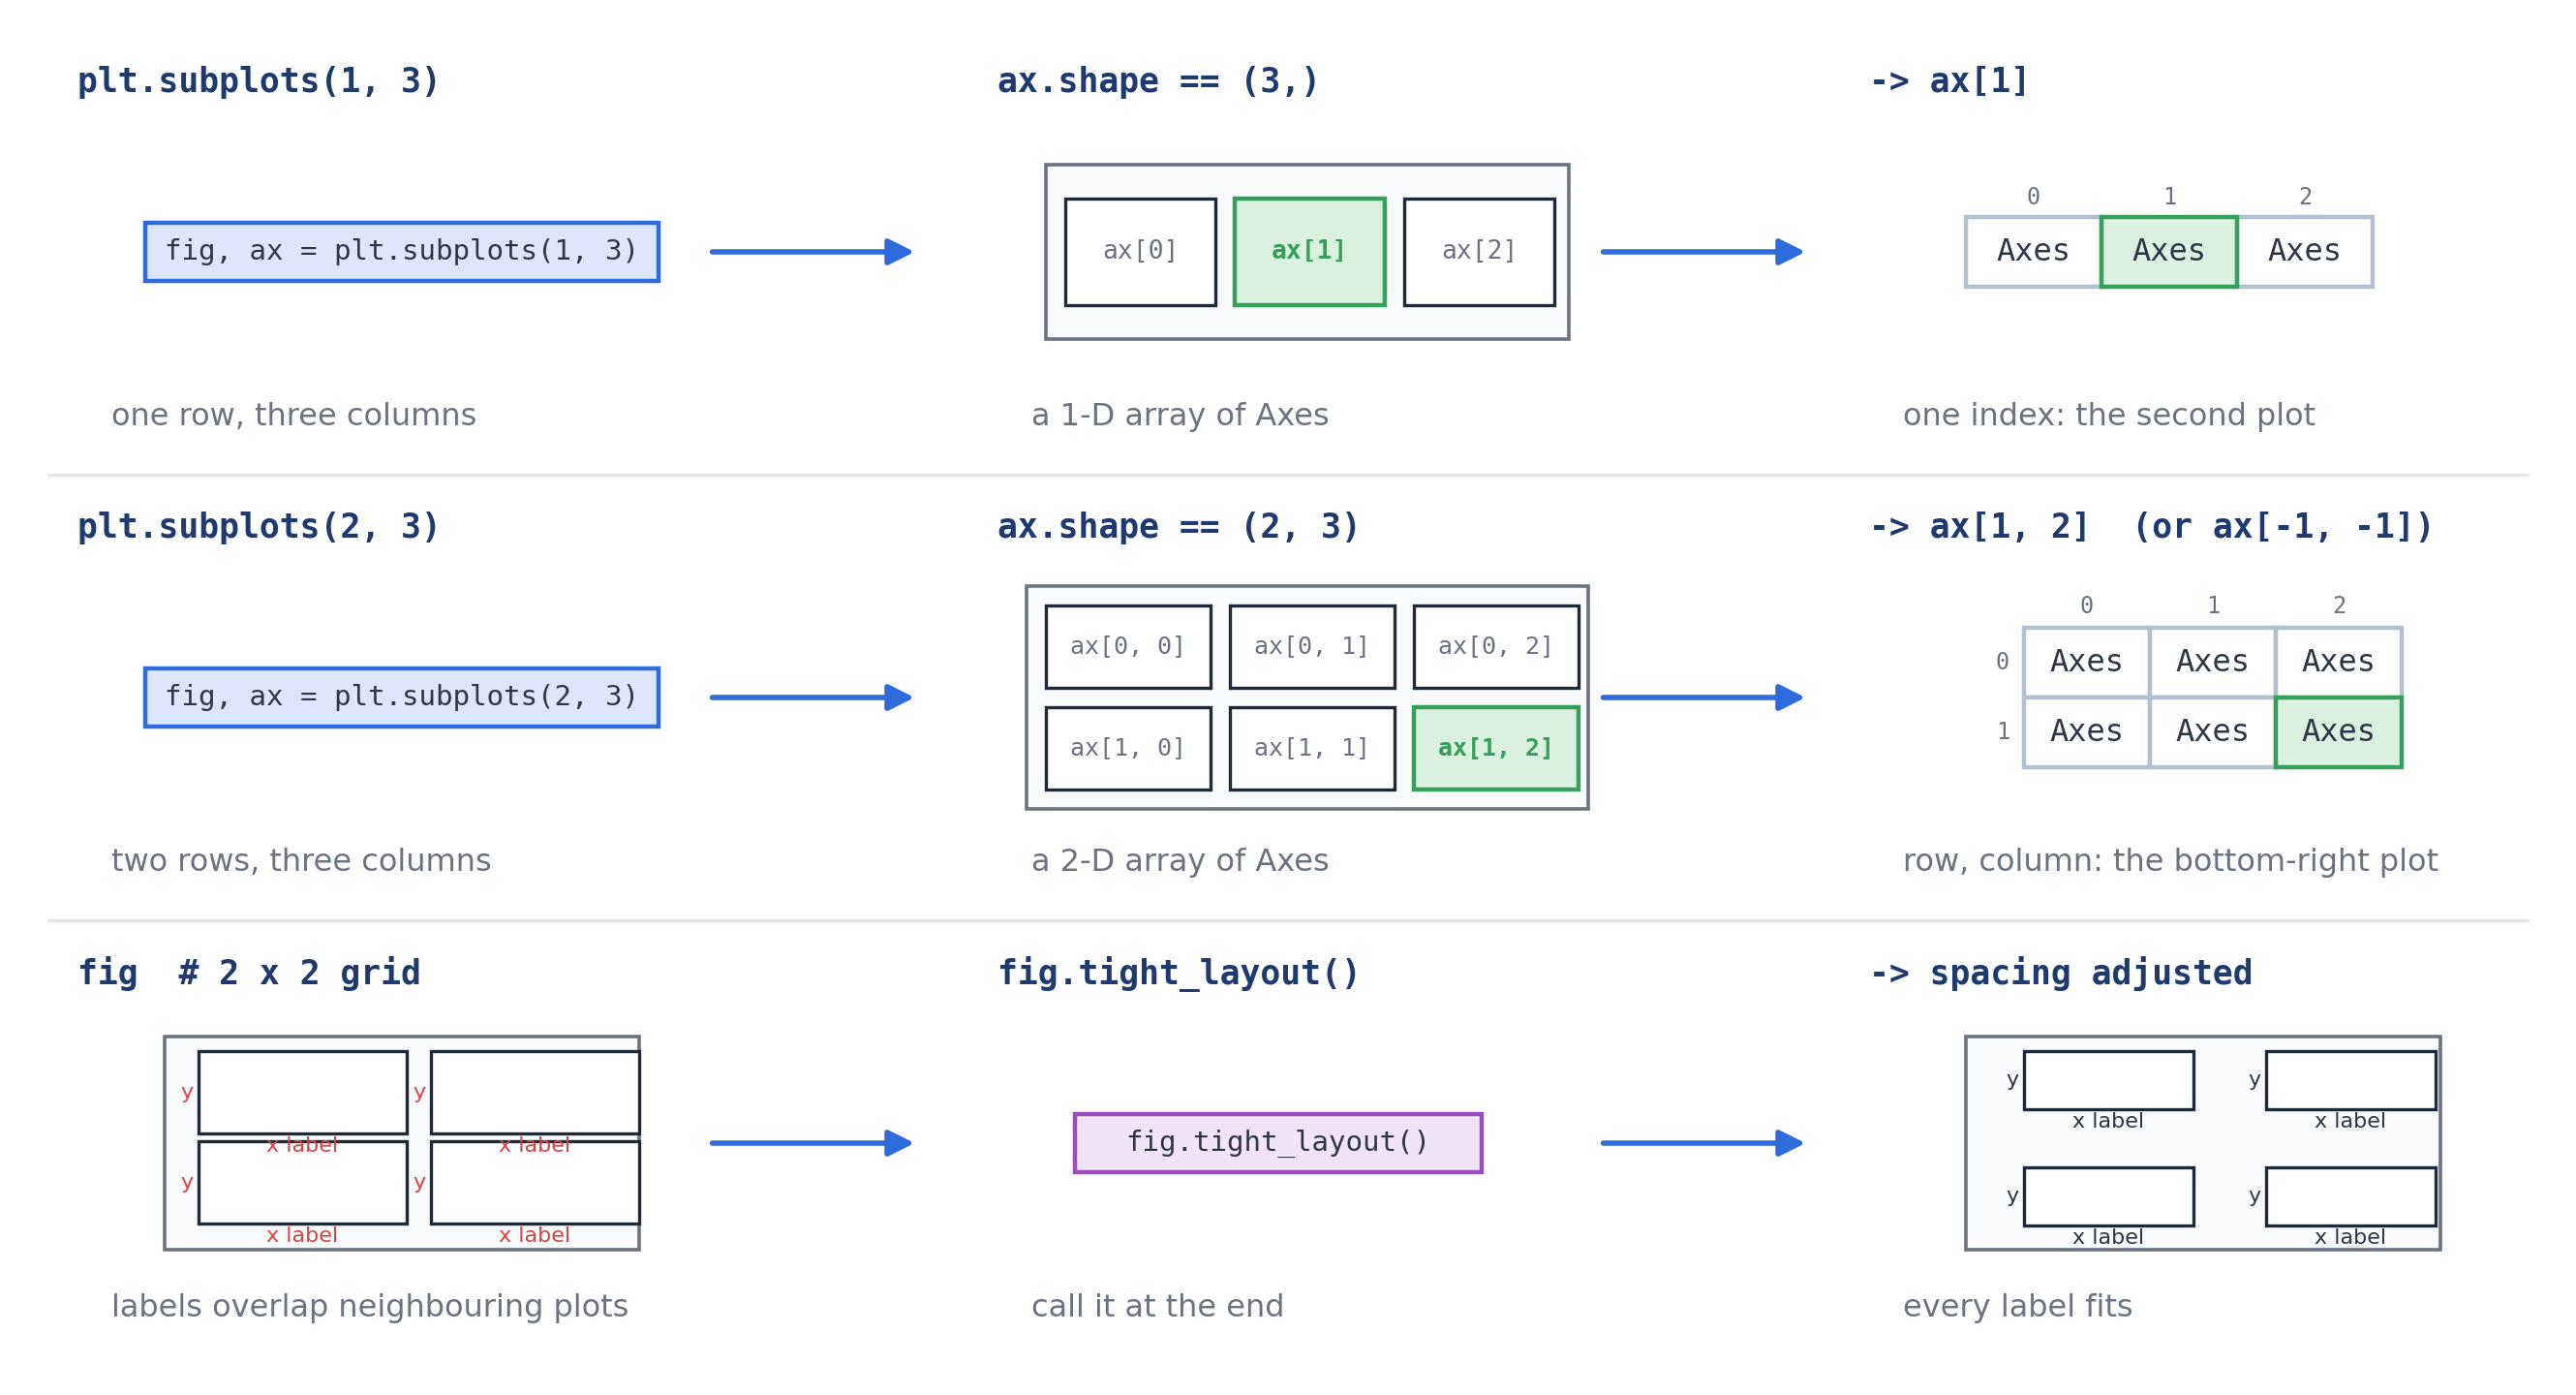
\includegraphics[width=1\textwidth]{contents/images/matplotlib/sub_subplots.png}
    \caption{Subplots: with one row, \texttt{ax} is a 1-D array indexed as \texttt{ax[j]}; with several rows and columns it is a 2-D array indexed as \texttt{ax[i, j]}. \texttt{fig.tight\_layout()} adjusts the spacing so that labels do not overlap.}
\end{figure}

\lstinputlisting[caption={Creating and managing 1D and 2D grids of subplots.}]{contents/listings/matplotlib/subplots.py}



\section{Plot Types}
Matplotlib provides various methods to visualize data. All of these methods are called directly on the \texttt{Axes} object (\texttt{ax}).

\subsection{Line and Scatter Plots}
\begin{itemize}
    \item \textbf{Line Plot (\texttt{ax.plot}):} Draws a sequence of points joined by segments, making it ideal for functions or time series[cite: 163, 171]. You can customize it using keyword arguments like \texttt{linestyle} (\texttt{'-'}, \texttt{'--'}, \texttt{':'}), \texttt{marker} (\texttt{'o'}, \texttt{'*'}), \texttt{color} (or \texttt{c}), and \texttt{label} (used to generate a legend).
    \item \textbf{Scatter Plot (\texttt{ax.scatter}):} Draws a cloud of independent points, useful for showing the relationship between two features. Unlike line plots, you can assign an individual color (\texttt{c}) and size/area (\texttt{s}) to every single point. Colors are usually mapped to numerical values using a colormap (\texttt{cmap}).
\end{itemize}

\begin{figure}[h]
    \centering
    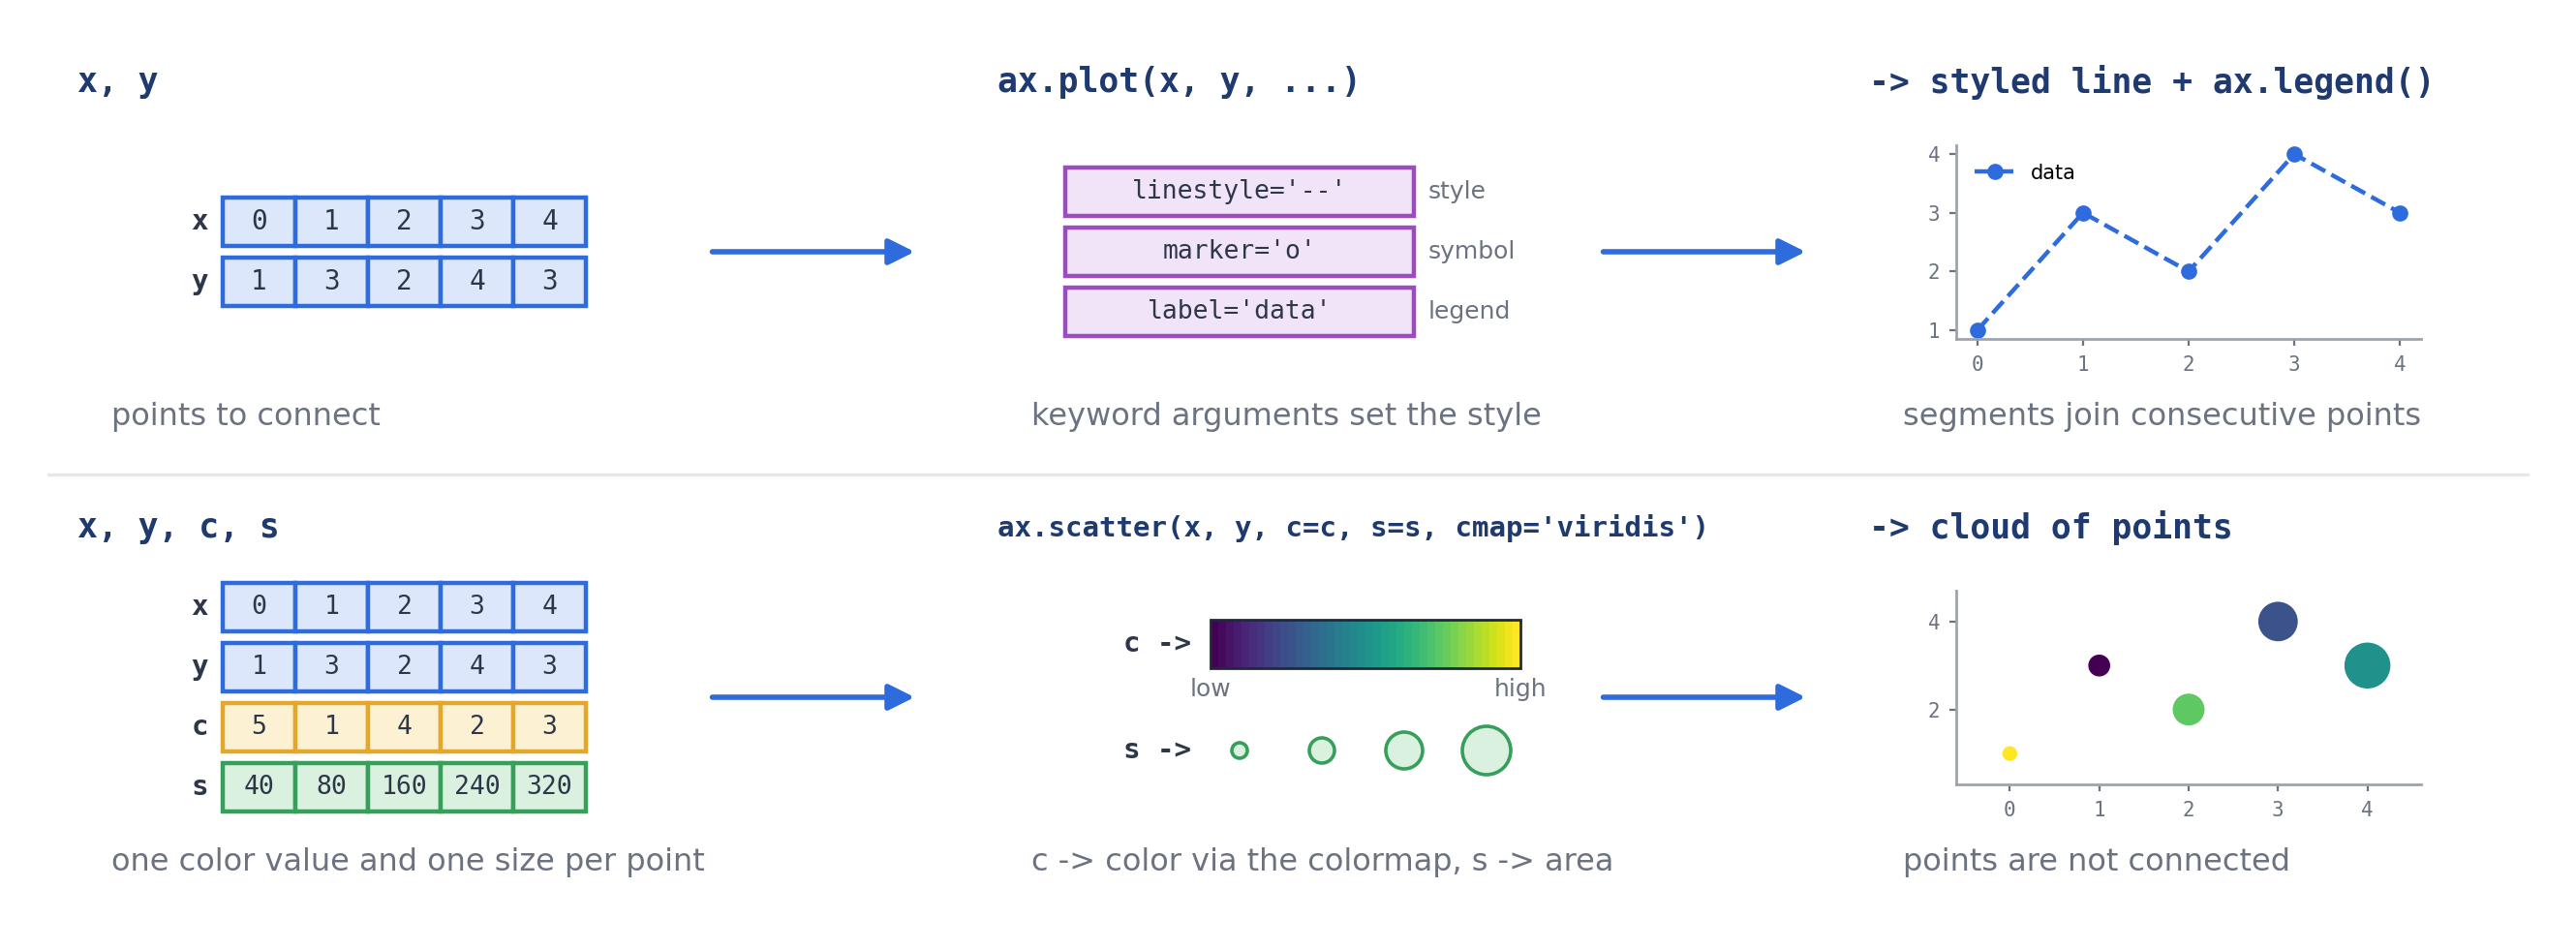
\includegraphics[width=1\textwidth]{contents/images/matplotlib/sub_line_scatter.png}
    \caption{Line and scatter plots: \texttt{ax.plot} joins consecutive points and is styled with keyword arguments such as \texttt{linestyle}, \texttt{marker} and \texttt{label}. \texttt{ax.scatter} draws unconnected points, each with its own color (\texttt{c}, mapped through \texttt{cmap}) and area (\texttt{s}).}
\end{figure}

\lstinputlisting[caption={Creating line plots and scatter plots with varying colors and sizes.}]{contents/listings/matplotlib/line_scatter.py}

\subsection{Bar Charts}
\begin{itemize}
    \item \textbf{Bar Chart (\texttt{ax.bar}):} Displays one numerical value per category. 
    \item To group multiple series of bars side-by-side, you can manually shift their positions along the x-axis (e.g., by subtracting or adding half the bar \texttt{width}) and update the ticks to show the category names.
\end{itemize}

\begin{figure}[h]
    \centering
    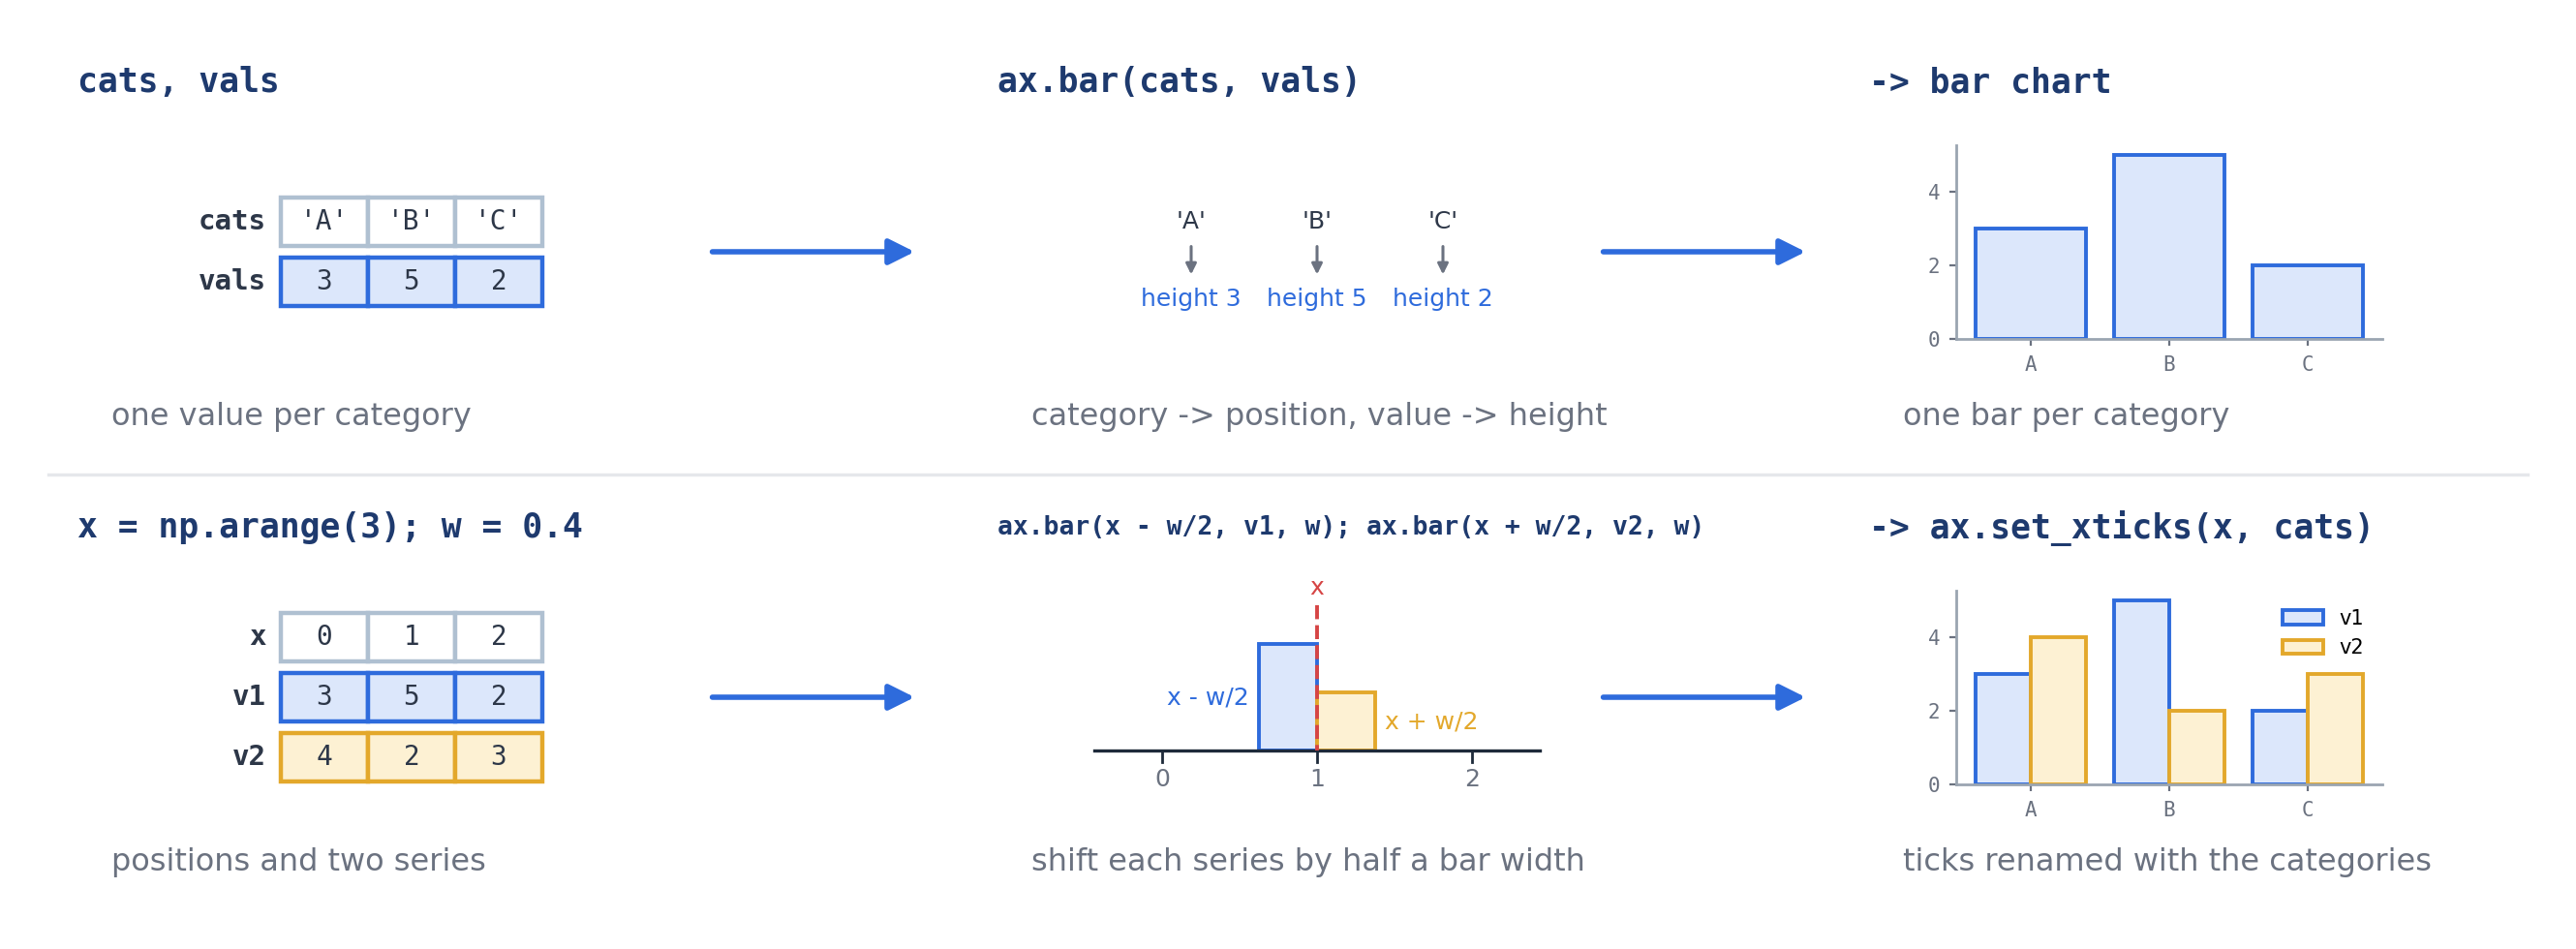
\includegraphics[width=1\textwidth]{contents/images/matplotlib/sub_bar.png}
    \caption{Bar charts: \texttt{ax.bar} draws one bar per category. To group two series, each is shifted by half a bar width around the integer positions \texttt{x}, and \texttt{ax.set\_xticks(x, cats)} puts the category names back on the axis.}
\end{figure}

\lstinputlisting[caption={Creating grouped bar charts.}]{contents/listings/matplotlib/bar.py}

\subsection{Histograms and Text Annotations}

\begin{figure}[h]
    \centering
    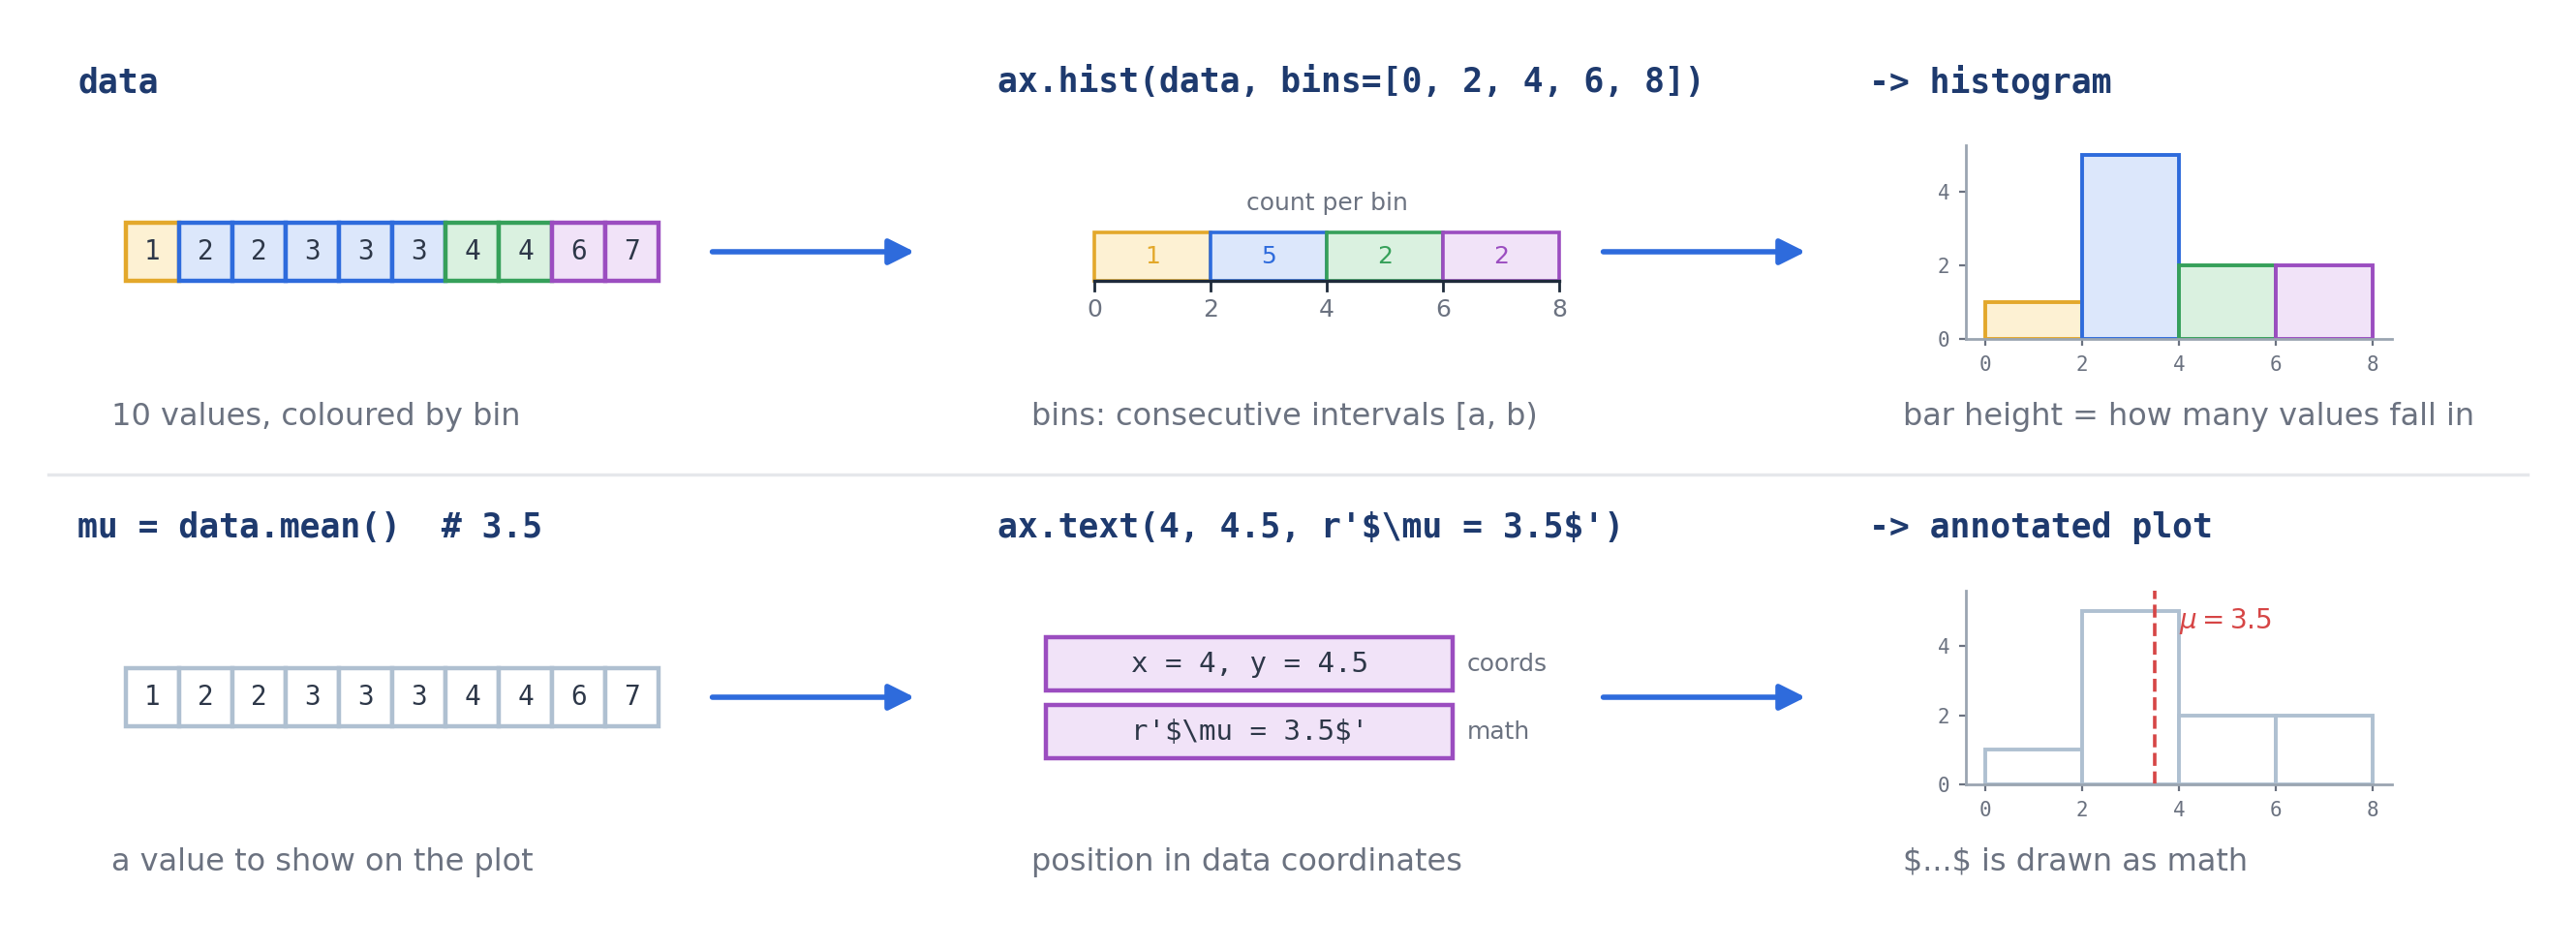
\includegraphics[width=0.85\textwidth]{contents/images/matplotlib/sub_hist_text.png}
    \caption{Histograms and annotations: \texttt{ax.hist} counts how many values fall into each bin (here with explicit edges), and \texttt{ax.text} writes a string at a position given in data coordinates, rendering the part between dollar signs as math.}
\end{figure}

\begin{itemize}
    \item \textbf{Histogram (\texttt{ax.hist}):} Shows the frequency distribution of a single variable, counting how many values fall into consecutive intervals (bins). The \texttt{bins} parameter can be an integer (to specify the number of equal bins) or a NumPy array defining the exact bin edges.
    \item \textbf{Annotations (\texttt{ax.text}):} You can write text directly on the plot by passing data coordinates (\texttt{x}, \texttt{y}). Matplotlib can render LaTeX math equations if the string is enclosed in dollar signs (e.g., \verb|$\mu$|).
\end{itemize}

\subsection{Box Plots}
\begin{itemize}
    \item \textbf{Box Plot (\texttt{ax.boxplot}):} Used to summarize and compare several distributions side-by-side.
    \item The central box extends from the first quartile (Q1) to the third quartile (Q3), with a line marking the median. 
    \item "Whiskers" extend outward to the farthest data points that fall within 1.5 times the Inter-Quartile Range (IQR). Any points beyond the whiskers are plotted as individual markers and are considered candidate outliers (fliers).
\end{itemize}

\begin{figure}[h]
    \centering
    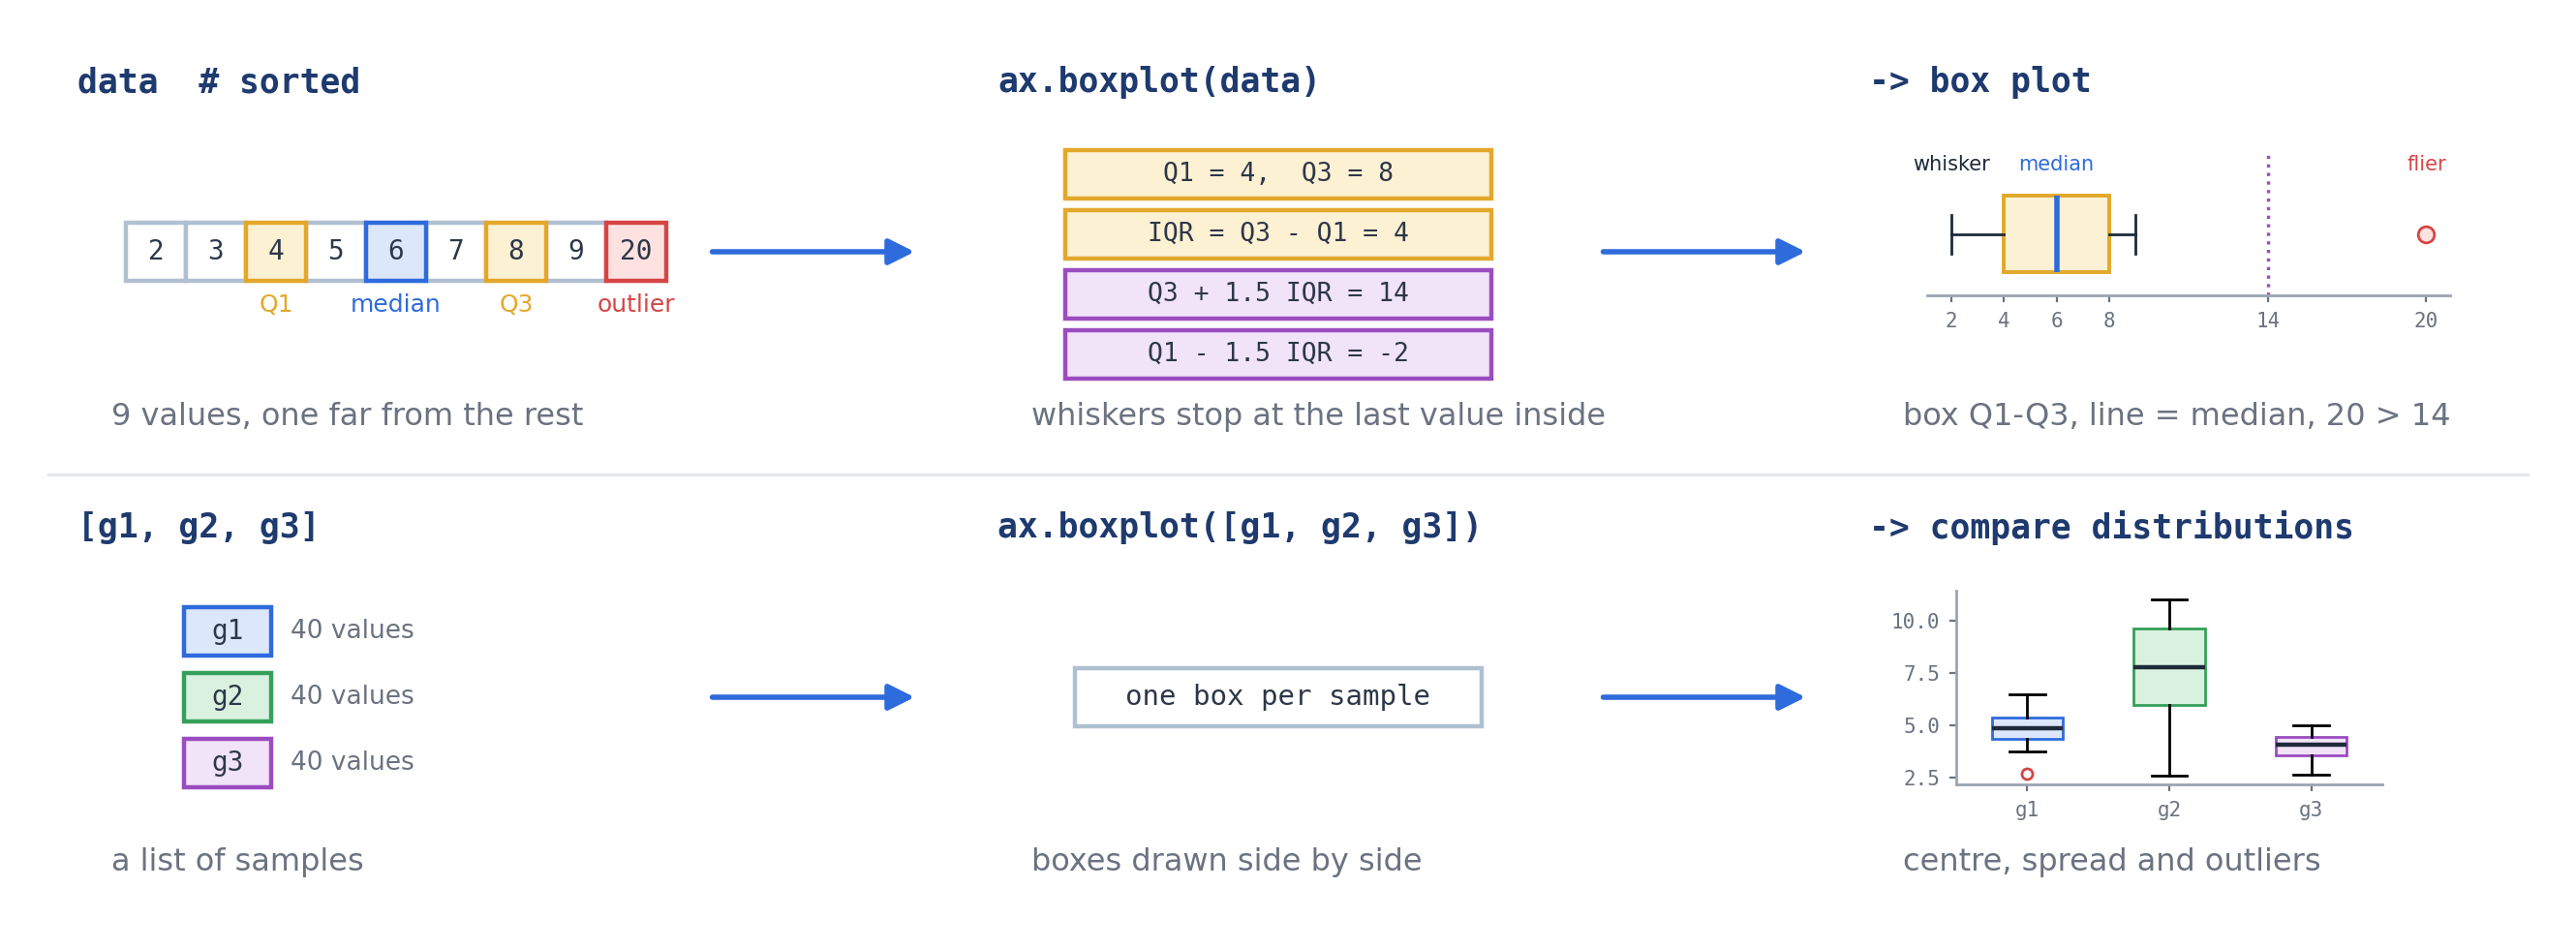
\includegraphics[width=1\textwidth]{contents/images/matplotlib/sub_boxplot.png}
    \caption{Box plots: the box spans Q1 to Q3 with a line at the median; the whiskers reach the farthest values within $1.5\,\mathrm{IQR}$ of the box, and values beyond are drawn as fliers. Passing a list of samples draws one box per sample for comparison.}
\end{figure}

\lstinputlisting[caption={Plotting histograms with text annotations and box plots.}]{contents/listings/matplotlib/hist_box.py}

\subsection{pandas Plotting Integration and Saving}

\begin{figure}[h]
    \centering
    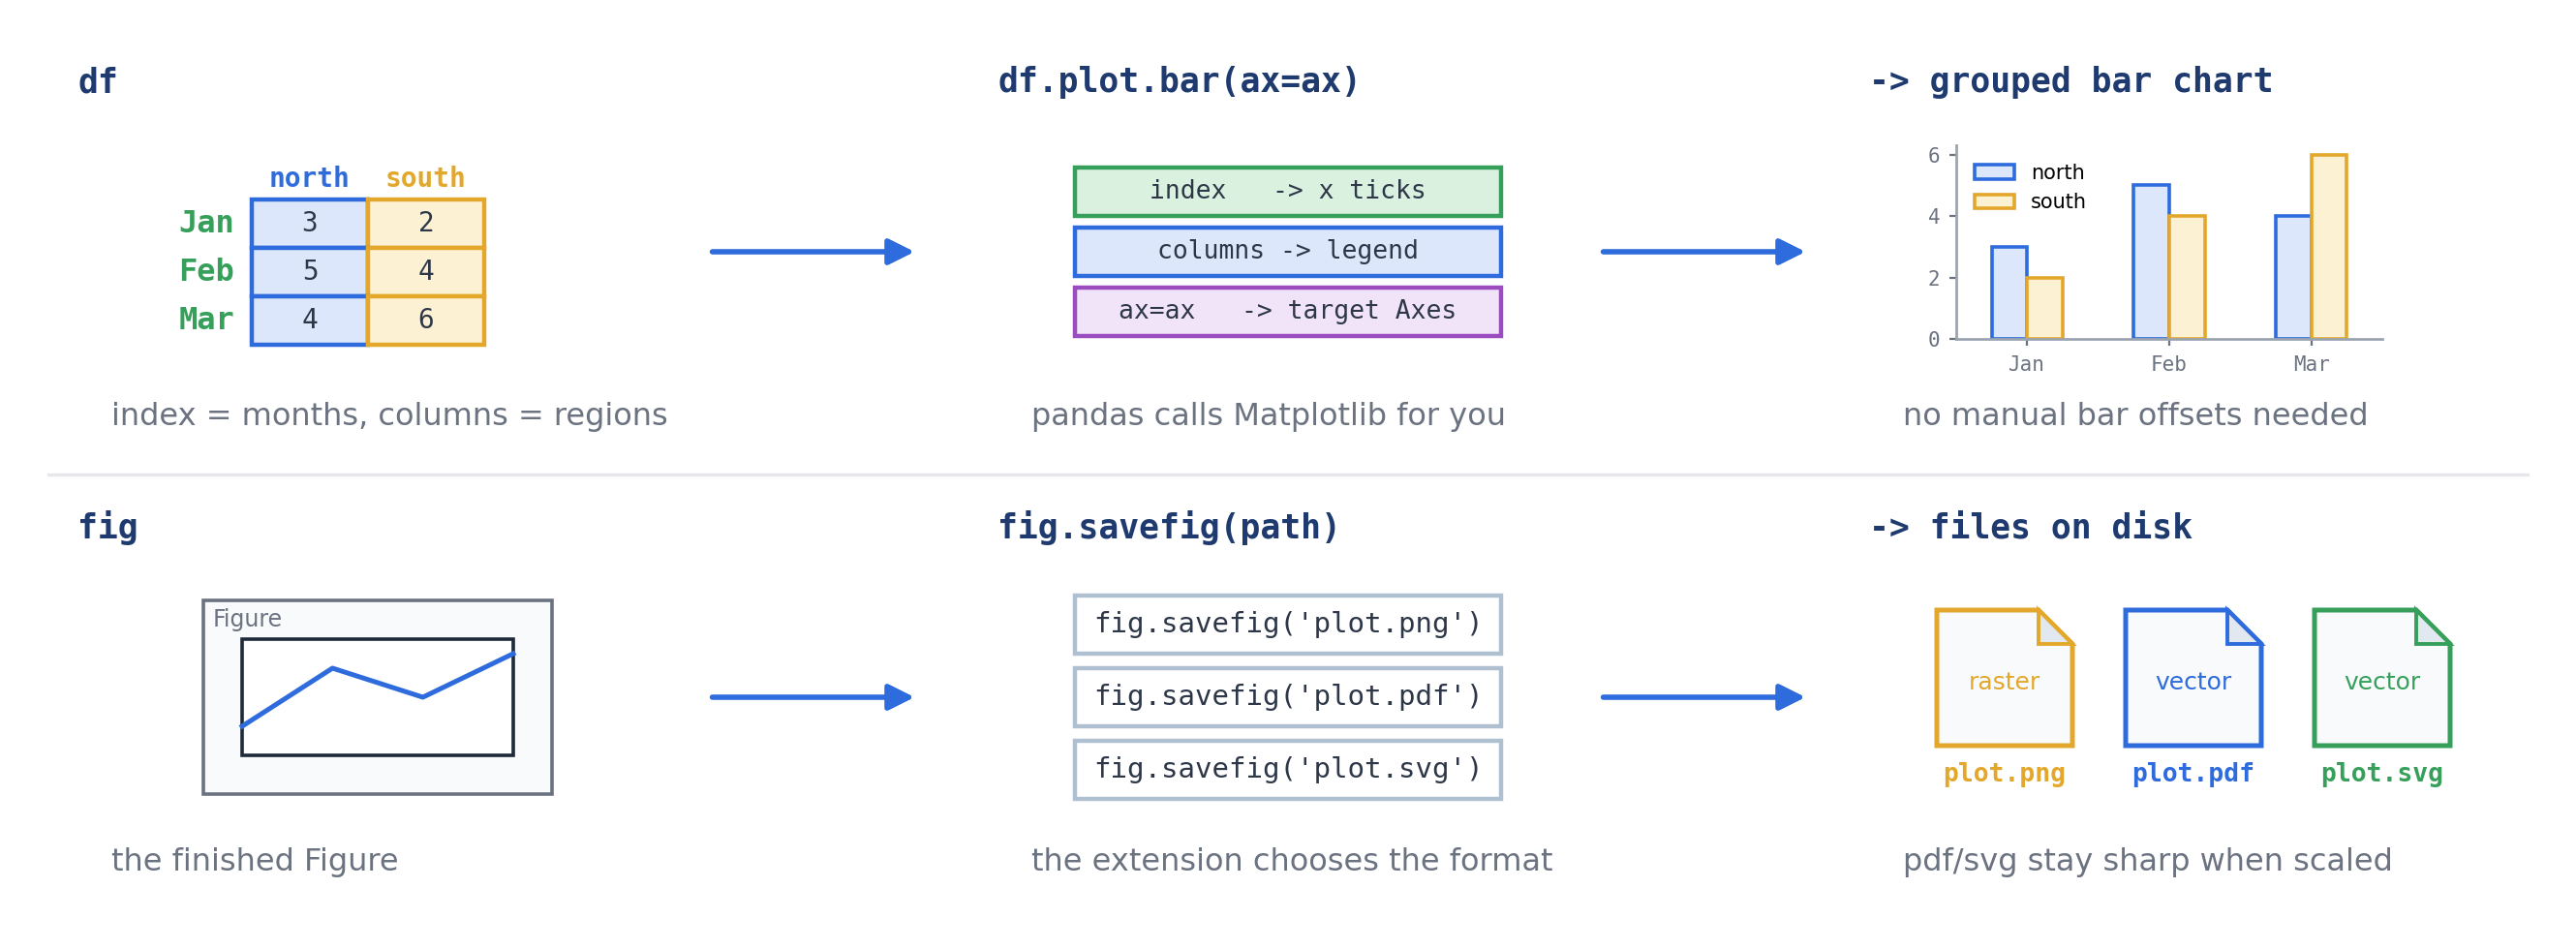
\includegraphics[width=1\textwidth]{contents/images/matplotlib/sub_pandas_plot.png}
    \caption{pandas plotting and saving: \texttt{df.plot.bar(ax=ax)} uses the index for the x-axis ticks and the column names for the legend, drawing on the given Axes. \texttt{fig.savefig} chooses the file format from the extension: PNG is a raster format, PDF and SVG are vector formats.}
\end{figure}

pandas Series and DataFrames have a built-in \texttt{.plot} accessor (e.g., \texttt{df.plot.bar()}) that automatically generates Matplotlib charts. It conveniently uses the DataFrame's index for the x-axis and its column names for the legend. By passing an \texttt{ax} argument (\texttt{ax=ax}), you can direct pandas to draw on your specific stateless Axes.

To save your final figure to disk, use \texttt{fig.savefig(path)}. Matplotlib automatically determines the file format based on the extension you provide (\texttt{.png}, \texttt{.pdf}, \texttt{.svg}, \texttt{.jpg}).





